\chapter{Random Number Generation} \label{sec:rng}

\section{Theory and Implementation}

\subsection{Random Telegraph Noise (RTN)}

The proposed RNG uses a device effect called Random Telegraph Noise (RTN) as the source of randomness. In general, RTN refers to the alternating capture and emission of carriers at a defect site (trap) of a very small electronic device, which generates discrete variation in the channel current \cite{kirton1989noise}. The capture and emission times are random and exponentially distributed. RTN behavior can be distinguished from other noise using the power spectrum density (PSD), which is flat at low frequencies and 1/f2 at high frequencies. In Flash memory, the defects that cause RTN are located in the tunnel-oxide near the substrate. The RTN amplitude is inversely proportional to the gate area and nearly temperature independent. As Flash memory cells shrink, RTN effects become relatively stronger and their impact on the threshold distribution of Flash memory cells, especially for multi-level cells, can be significant. Because RTN can be a major factor in Flash memory reliability, there have been a large number of recent studies on RTN in Flash memory from a reliability perspective \cite{kurata2007random, compagnoni2009random, joe2011threshold}.
While RTN is a challenge to overcome from the perspective of Flash memory operations, it can be an ideal source of randomness. RTN is caused by the capture and emission of an electron at a single trap, and is a physical phenomenon with random quantum properties. Quantum noise can be seen as the “gold-standard” for random number generation because the output of quantum events cannot be predicted. As Flash memory cells scale to smaller technology nodes, the RTN effect will become stronger. Moreover, RTN behavior will still exist with increasing process variation and at extremely low temperatures. 

\subsection{Noise Extraction from Digital Interface}

As digital devices, Flash memory is designed to tolerate analog noise; noise should not affect normal memory operations. In order to observe the noise for random number generation, a Flash cell needs to be in an unreliable state between well-defined erase and program states. Interestingly, we found that Flash cells can be put into the in-between state using the standard digital interface. In a high level, the approach first erases a page, issues a program command, and then issues a reset command after an appropriate time period to abort the program. This procedure leaves a page partially programmed so that noise can affect digital outputs. We found that the outcome of continuously reading a partially programmed bit oscillates between 1 and 0 due to noise. 

\begin{figure} 
\begin{center} 
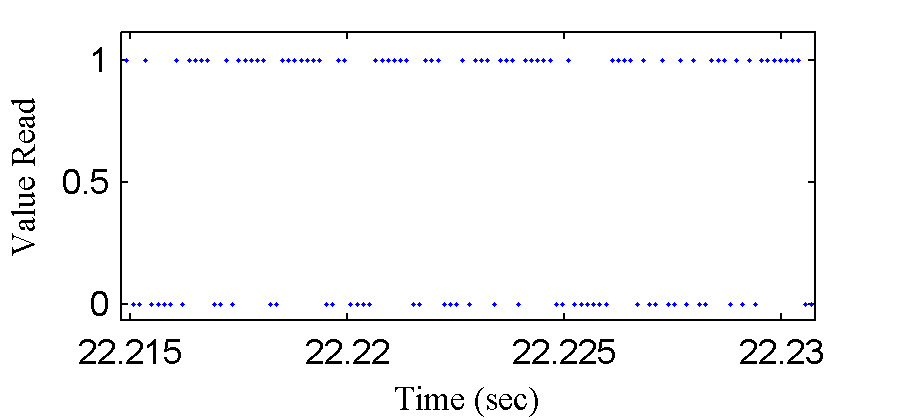
\includegraphics[width=\mywidth]{figs/thermal_noise.png} 
%\includegraphics[width=3.0in]{figs/eval_performance_diff_context.pdf} 
\caption{Thermal noise in Flash memory (time domain).}
\label{fig:thermal} 
\vspace{-0.25in}
\end{center} 
\end{figure} 

For Flash memory in practice, experiments show that two types of noise coexist: thermal noise and RTN. Thermal noise is white noise that exists in nearly all electronic devices. RTN can be observed only if a surface trap exists, the RTN amplitude is larger than that of thermal noise, and the sampling frequency (speed for continuous reads) is high enough. If any of these three conditions is not satisfied, only thermal noise will be observed as in Figure~\ref{fig:thermal}. In the case of thermal noise, a bit oscillates between the two states quickly, and the power spectral density (PSD) indicates white noise. 

\begin{figure}
  \centering
  \subfigure[][]{
    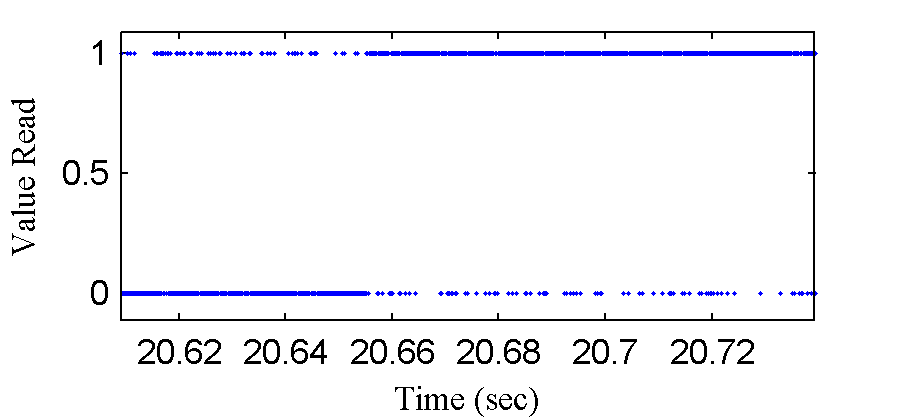
\includegraphics[width=\mywidth]{figs/thermal_rng_noise1.png}
    \label{fig:thermal_rtn1}
  }
  
  \subfigure[][]{
    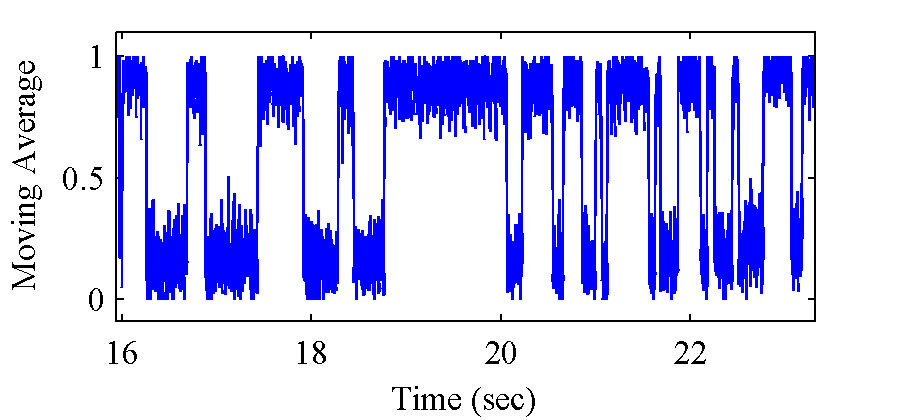
\includegraphics[width=\mywidth]{figs/thermal_rng_noise2.png}
    \label{fig:thermal_rtn2}
  }
  \caption{RTN with thermal noise in Flash memory. (a) Time domain. (b) Moving average of 29 points on the time domain.}
  \label{fig:thermal_rtn}
\end{figure}

In the case that the RTN amplitude is comparable to thermal noise, a combination of RTN and thermal noise is observed as shown in Figure~\ref{fig:thermal_rtn}. This is reflected by the density change of 1s in the continuous reading. A moving average on the time domain helps to visualize the density change. The PSD of the result shows $1/{f}^2$ spectrum at low frequencies and becomes flat at high frequencies.

\begin{figure} 
\begin{center} 
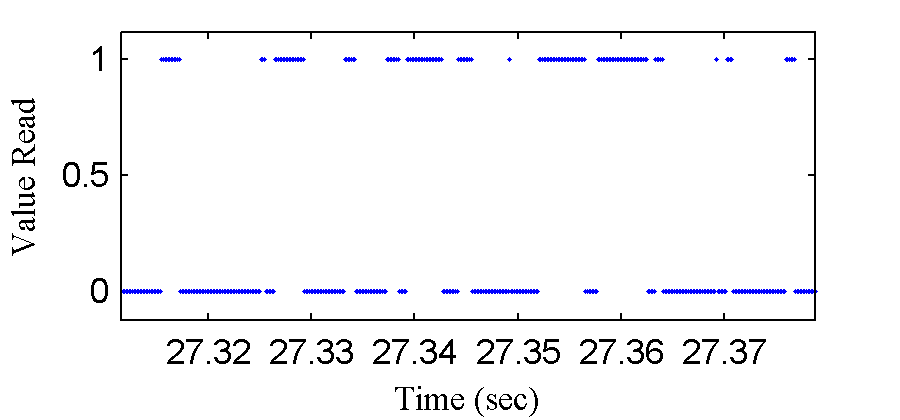
\includegraphics[width=\mywidth]{figs/rtn.png} 
%\includegraphics[width=3.0in]{figs/eval_performance_diff_context.pdf} 
\caption{RTN in Flash memory (time domain).}
\label{fig:rtn} 
\vspace{-0.25in}
\end{center} 
\end{figure} 

In some cases, the RTN amplitude is very high and dominates thermal noise. As a result, only RTN behaviors are visible through digital interfaces for these bits. As shown in Figure~\ref{fig:rtn}, continuous reads show clear clusters of 1s and 0s in the time domain. The power spectral density (PSD) of these bit sequences shows a clear RTN pattern of $1/{f}^2$. 

 
\begin{figure}
  \centering
  \subfigure[][]{
    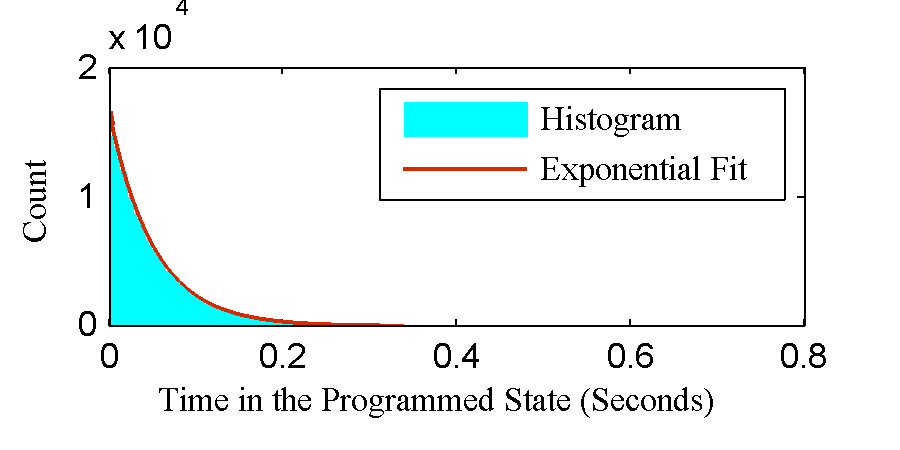
\includegraphics[width=\mywidth]{figs/rtn_freq_pstate.png}
    \label{fig:rtn_freq_pstate}
  }
  
  \subfigure[][]{
    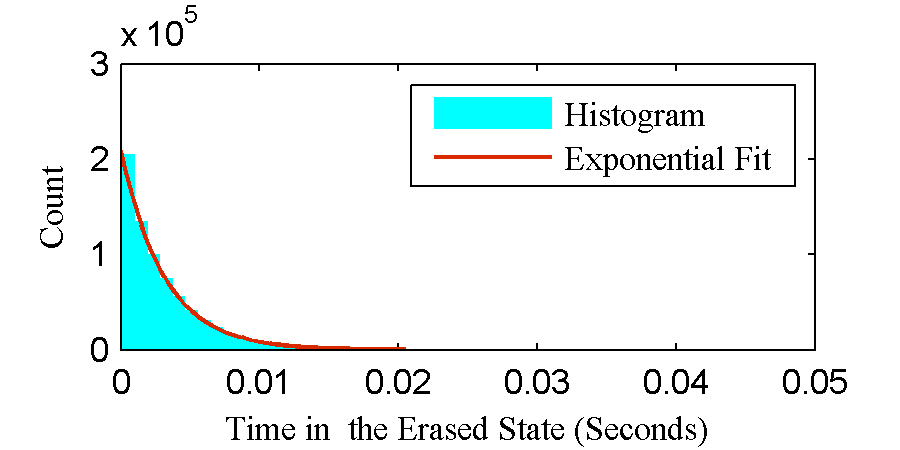
\includegraphics[width=\mywidth]{figs/rtn_freq_estate.png}
    \label{fig:rtn_freq_estate}
  }
  \caption{(a) Distribution of time in the programmed state. 
(b) Distribution of time in the erased state.}
  \label{fig:rtn_freq}
\end{figure}


For a bit with nearly pure RTN behavior, we further validated that the error pattern corresponds to RTN by plotting the distributions of up and down periods. As shown in Figure~\ref{fig:rtn_freq}, both up time and down time nicely fit an exponential distribution as expected. Overall, our experiments show that both RTN and thermal noise exist in Flash memory and can be observed through a digital interface. While both noise types can be used for random number generation, we focus on RTN, which is more robust to temperature changes.

\subsection{Random Number Generation Algorithms}

In Flash memory devices, RTN manifests as random switching between the erased state (consecutive 1s) and programmed state (consecutive 0s). At a high-level, our Flash random number generator (RNG) identifies bits with RTN behavior, either pure RTN or RTN combined with thermal noise, and uses a sequence of time in the erased state (called up-time) and the time in the programmed state (called down-time) from those bits. In order to produce random binary outputs, the RNG converts the up-time and down-time sequence into a binary number sequence, and applies the von Neumann extractor for de-biasing. We found that thermal noise itself is random and does not need to be filtered out.

\begin{figure} 
\begin{center} 

%\begin{scriptsize}
\begin{center}

\begin{tabular}{|c|}
\hline
\begin{minipage}[t]{3.2in}



\begin{tabbing}
{\bf Algorithm I  Overall Flash RNG algorithm }
\\
\\ Erase a block;
\\
\\ Num = 0;
\\ do \=
\\ \>Partially program a page for T;
\\ \>Num++;
\\
\\ \>Read Nbytes in a page N times, and record a 
\\ \>trace for each bit – trace[bit];
\\ \>{\bf For} \= each bit in Nbytes, not selected yet
\\ \>\>{\bf    If} \= (CheckRTN(trace[bit]) == true) 
\\ \>\>\>          Selected[bit] = yes;
\\ \>\>\>          NumProgram[bit] = Num;
\\ \>{\bf End for}
\\ \> repeat until most bits are programmed.
\\
\\ ProgramSelectBits(Selected);
\\
\\ Read selected bits M times, and record up-time and down-time;
\\ {\bf For} \= each bit
\\ \>      ConvertToBinary(rawdata);
\\ {\bf End for}


\end{tabbing}
\end{minipage}
\\ \hline
\end{tabular}
\end{center}
%\end{scriptsize}
 
\caption{Overall Flash RNG algorithm}
\label{fig:overal_rng_al} 
\vspace{-0.25in}
\end{center} 
\end{figure}

Algorithm I shows the overall RNG algorithm. To generate random numbers from RTN, the first step is to identify bits with RTN or both RTN and thermal noise. To do this, one block in Flash memory is erased and then multiple incomplete programs with the duration of T are applied. After each partial program, a part of the page is continuously read N times and the outcome is recorded for each bit. In our experiments, we chose to read the first 80 bits (10 bytes) in a page for 1,000 times. For each bit that has not been selected yet, the algorithm checks if RTN exists using CheckRTN() and marks the bit location if there is RTN. As an optimization, the algorithm also records the number of partial programs when a bit is selected. The algorithm repeats the process until all bits are checked for RTN. The second step is to partially program all of the selected bits to an appropriate level so that they will show RTN behavior. Finally, the algorithm reads the selected bits M times, records a sequence of up-time and down-time for each bit, and converts the raw data to a binary sequence. 

\begin{figure} 
\begin{center} 

%\begin{scriptsize}
\begin{center}

\begin{tabular}{|c|}
\hline
\begin{minipage}[t]{3.2in}



\begin{tabbing}
{\bf Algorithm II  Determine whether there is RTN in a bit }
\\
\\ {\bf If} \= trace[bit] has over 98\% 1/0s
\\ \>        {\bf Return} false;
\\ {\bf End if} 
\\
\\ Calculate the power spectrum density (PSD);
\\ Convert PSD to the log scale in both x-y;

\\ {\bf If} \= PSD slope is always $< T_{slope}$ for all high frequency ($> T_{freq}$)
\\ \> {\bf Return} RTN
\\ {\bf End if} 
\\
\\ {\bf If} \= PSD slope is $< T_{slope}$ at least one interval (Invl) at a high frequency ($> T_{freq}$)
\\ \> {\bf Return} RTN-Thermal
\\ {\bf End if}


\end{tabbing}
\end{minipage}
\\ \hline
\end{tabular}
\end{center}
%\end{scriptsize}
 
\caption{Determine whether there is RTN in a bit}
\label{fig:rtn_bit} 
\vspace{-0.25in}
\end{center} 
\end{figure}

The function CheckRTN() in Algorithm II determines whether there is RTN in a bit based on a trace from N reads. The algorithm first filters out bits that almost always (more than 98\%) produce one result, either 1 or 0. For the bits with enough noise, the algorithm uses the power spectral density (PSD) to distinguish RTN from thermal noise; PSD for RTN has a form of $1/{f}^2$ at a high frequency. To check this condition, the algorithm computes the PSD, and converts it to a log-scale in both x and y axes. If the result has a slope less than Tslope (we use -1.5, the ideal value is -2) for all frequencies higher than Tfreq (we use 200Hz), the algorithm categorizes the bit as RTN only. If the PSD has a slope less than Tslope for any interval larger than than Invl (we use 0.2) at a high frequency, the bit is categorized as a combination of RTN and thermal noise.

\begin{figure} 
\begin{center} 

%\begin{scriptsize}
\begin{center}

\begin{tabular}{|c|}
\hline
\begin{minipage}[t]{3.2in}



\begin{tabbing}
{\bf Algorithm III  Program selected bits to proper levels }
\\ {\bf where RTN could be observed. }
\\
\\ {\bf For} \= each selected bit
\\ \> Do (NumProgram[bit]-K) partial programs;
\\
\\ \> {\bf do} \= \{
\\ \>\>  Partially program the bit for T;
\\
\\ \>\>  Read the bit N times;
\\ \>\>  Find Max and Min for moving averages;
\\
\\ \>\> {\bf If} \= $Max > TMax$ and $Min < TMin$ 
\\ \>\>\>    Break;
\\ \>\> {\bf End if}
\\ \> \} repeat up to L times
\\ {\bf End for}


\end{tabbing}
\end{minipage}
\\ \hline
\end{tabular}
\end{center}
%\end{scriptsize}
 
\caption{Program selected bits to proper levels where RTN could be observed.}
\label{fig:prg_rtn} 
\vspace{-0.25in}
\end{center} 
\end{figure}

The function ProgramSelectBits() in Algorithm III programs selected bits to a proper level where RTN can be observed. Essentially, the algorithm aims to take each bit to the point near where they were identified to have RTN. The number of partial programs that were required to reach this point before were recorded in NumProgram[Bit]. For each selected bit, the algorithm first performs partial programs with the duration of T based on the number recorded earlier (NumProgram[Bit]-K). Then, the algorithm performs up to L more partial program operations until a bit shows RTN behavior. The RTN behavior is checked by reading the bit N times, and see if the maximum of moving averages is greater than a threshold ($TMax = 0.7$) and the minimum is less than another threshold ($TMin = 0.3$). 

\begin{figure} 
\begin{center} 

%\begin{scriptsize}
\begin{center}

\begin{tabular}{|c|}
\hline
\begin{minipage}[t]{3.2in}



\begin{tabbing}
{\bf Algorithm IV Convert the raw data to binary random sequence. }
\\
\\ {\bf If} \= the bit has both RTN and thermal noise
\\ \> {\bf For} \= each up/down-time in raw data
\\ \>\>   Output = LSB(up/down-time);
\\ \> {\bf End for}
\\ {\bf End if}
\\
\\ {\bf If} \= the bit has only RTN
\\ \> {\bf do} \= \{
\\ \>\> {\bf For} \= each up/down-time in raw data
\\ \>\>\>    Output = LSB(up/down-time);
\\ \>\>\>    Shift right up/down-time by one bit;
\\ \>\> {\bf End for}
\\ \> \} repeat until all up/down time are zero;
\\ {\bf End if}
\\
\\Perform von Neumann de-biasing


\end{tabbing}
\end{minipage}
\\ \hline
\end{tabular}
\end{center}
%\end{scriptsize}
 
\caption{Convert the raw data to binary random sequence.}
\label{fig:to_bin_seq} 
\vspace{-0.25in}
\end{center} 
\end{figure}

Finally, the function ConvertToBinary() converts the raw data to a binary random sequence. For bits with both RTN and thermal noise, the up-time and down-time tend to be short. So only the LSBs of these numbers are used. Essentially, for every up-time and down-time, the algorithm produces 1 if the time is odd and 0 otherwise. Effectively, this is an even-odd scheme. For bits with perfect RTN behavior, up-time and down-time tend to be longer and we use more LSBs from the recorded up/down-time. In this case, we first produce a bit based on the LSB, then the second LSB, the third LSB, and so on until all extracted bits become 0. Finally, for both methods, we apply the von Neumann de-biasing method. The method takes two bits at a time, throws away both bits if they are identical, and takes the first bit if different. This process is described in Algorithm IV.

The stability of the bits in the partially programmed state is also important. We define the stability as how long a bit stays in the partially programmed state where RTN behavior can be observed. This is determined by the retention time of the Flash memory chip and the amplitude of the RTN compared to the designed noise margin. Assume the amplitude of the RTN is Ar, the noise margin of Flash memory is An, and the Flash retention time is 10 year, then the stable time for random number generation after partial programming will be roughly $Ts=Ar/An*10$ years. This means that after time Ts, a bit needs to be reset and reprogrammed. In our experiments, the bit that is shown in Figure~\ref{fig:rtn_freq} was still showing ideal RTN behavior even after 12 hours.

\section{Experimental Results}

This section presents evaluation results for the random number generation techniques for Flash memory devices. The two main metrics for random number generation are randomness and throughput. For security, the RNG must be able to reliably generate true random numbers across a range of environmental conditions over time. For performance, higher throughput will be desirable. 

\subsection{Evaluation Setup}

\begin{figure}
\begin{center} 
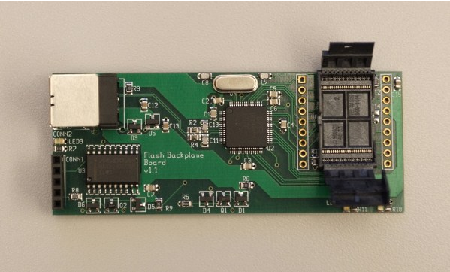
\includegraphics[width=\mywidth]{figs/flashtestboard.pdf} 
\caption{Flash test board.}
\label{fig:flashtestboard} 
\vspace{-0.1in}
\end{center} 
\end{figure} 

Our experiments use a custom Flash test board as shown in 
Figure~\ref{fig:flashtestboard}. The board is made entirely with 
commercial off-the-shelf (COTS) components with a custom PCB. 
There is a socket to hold a Flash chip under test, an ARM 
microprocessor to issue commands and receive data from the Flash 
chip, and a Maxim MAX-3233 chip to provide a serial (RS-232) 
interface. USB support is integrated into the ARM microcontroller. 
We also wrote the code to test the device. The setup represents 
typical small embedded platforms such as USB Flash drives, sensor 
nodes, etc. This device shows that the techniques can be applied 
to commercial off-the-shelf devices with no custom integrated 
circuits (ICs).

\begin{table}
  \begin{center}
    %\begin{scriptsize}
\begin{tabular}{|l|l|r|r|r|}
\hline

{\bf Manufacturer}& {\bf Part Number} & {\bf Size} & {\bf Qty} & {\bf Process} \\

\hline
Hynix & HY27UF084G2B & 4 Gbit & 10 & 5xnm class\\
       & & & & SLC\\
\hline
Micron & MT29F2G08ABA & 2 Gbit & 24 & 34nm \\
       & EAWP-IT:E4 & & & SLC\\
\hline
Micron & MT29F16G08CB & 16 Gbit & 5 & -- \\
       & ACAWP:C & & & MLC\\
\hline
Numonyx & NAND04GW & 4 Gbit & 3 & 57nm \\
& 3B2DN6 & & & SLC\\
 
\hline

\end{tabular}
%\end{scriptsize}
  \end{center}
\caption{Tested Flash chips.}
\vspace{-0.2in}
\label{tab:testedchips}
\end{table}

The experiments in this paper were performed with four types of Flash memory chips from Numonyx, Micron and Hynix, as shown in Table~\ref{tab:testedchips}.

\subsection{ Randomness}

Historically, three main randomness test suites exist. The first one is from Donald Knuth’s book “The Art of computer Programming (1st edition, 1969)” \cite{knuth1973art} which is the most quoted reference in statistical testing for RNGs in literature. Although it was a standard for many decades, it appears to be outdated in today’s view and it allows many “bad” generators to pass the tests. The second one is the “diehard” test suite from Florida State University. The test suite is stringent in the sense that they are difficult to pass. However, the suite has not been maintained in recent years. Therefore, it was not selected as the tests for this study. The third one is developed by National Institute of Standards and Technology (NIST) which is a measurement standard laboratory and a non-regulatory agency of the United States Department of Commerce. The NIST Statistical Test Suite is a package consisting of 15 tests that were developed to test the randomness of arbitrary long binary sequences produced by either hardware or software. The test suite makes use of both existing algorithms from past literatures and newly developed tests. The most updated version, sts-2.1.1, which was released in August 11, 2010, is used in our randomness tests. TABLE~\ref{tab:nist} summarizes the 15 NIST tests \cite{rukhin2001statistical}.

\begin{table}
  \begin{center}
    %\begin{scriptsize}
\begin{tabular}{|l|l|}
\hline

{\bf Test Name}& {\bf Test Description} \\

\hline
1 The Frequency & Tests proportion of zeros and \\
(Monobit) Test & ones for the whole sequence.\\
\hline
2 Frequency Test  & Tests the proportions of ones\\
within a Block    & within M-bit Block.\\
\hline
3 The Run Test & Tests the total number of runs in the \\
               & sequence, where a run is an uninterrupted \\
               & sequence of identical bits \\
\hline
4 Tests for the Longest- & Tests the longest run of ones within M-bit \\
Run-of-Ones in a Block & Block and consistency with theory \\
\hline
5 The Binary Matrix & Tests rank of disjoint sub-matrices \\
Rank Test & of the entire sequence and independence \\
\hline
6 The Discrete Fourier & Tests the peak heights in the Discrete Fourier  \\
Transform (Spectral) Test & Transform of the sequence, to detect periodic \\
                       & features that indicates deviation of randomness \\
\hline
7 The Non-overlapping & Tests the number of occurrences of\\
Template Matching Test & a pre-specified target strings \\
\hline
8 The Overlapping & Tests the number of occurrences of a \\
Template Matching Test & pre-specified target strings. When window \\
                   & found, slide only one bit before the next search \\
\hline
9 Maurer’s “Universal & Tests the number of bits \\
Statistics” Test & between matching patterns \\
\hline
10 The Linear & Tests the length of a linear feedback \\
Complexity Test & shift register, test complexity \\
\hline
11 The Serial Test & Tests the frequency of all \\
                  & possible overlapping m-bit pattern \\
\hline
12 The Approximate & Tests the frequency of all possible overlapping\\
Entropy Test &  m-bits pattern across the entire sequence \\
\hline
13 The Cumulative & Tests maximal excursion from the random walk \\
Sums (Cusums) Test & defined by the cumulative sum of adjusted \\
                  & (-1, +1) digits in the sequence \\
\hline
14 The Random & Tests the number of cycles having exactly K \\
Excursion Test & visits in a cumulative sum random walk \\
\hline
15 The Random Excursions & Tests the total number of times that a particular \\
Variant Test & state is visited in a cumulative sum random walk  \\

 
\hline

\end{tabular}
%\end{scriptsize}
  \end{center}
\caption{Summary of the NIST test suite}
\vspace{-0.2in}
\label{tab:nist}
\end{table}

Figure~\ref{fig:nist_result} shows one test result for the even-odd scheme, which only used an LSB from the up-time and down-time, when bits with both RTN and thermal noise are used. 10 sequences generated from multiple bits are tested and each sequence consists of 600,000 bits. Note that some of the results are not shown here due to the space constraint.  NonOverlappingTemplate, RandomExcursions and RandomExcursionsVariant have a lot of tests. In the result above, the proportion in the second column shows the proportion of the sequences which passed the test. If the proportion is greater than or equal to the threshold value specified at the bottom of the figure (8 out of 10 or 4 out of 5), then the data is considered random. The P-value in the first column indicates the uniformity of the P-values calculated in each test. If P-value is greater than or equal to 0.0001, the sequences can be considered to be uniformly distributed \cite{rukhin2001statistical}. The result indicates that the proposed RNG passes all the NIST tests. 

\begin{figure}
\begin{center} 
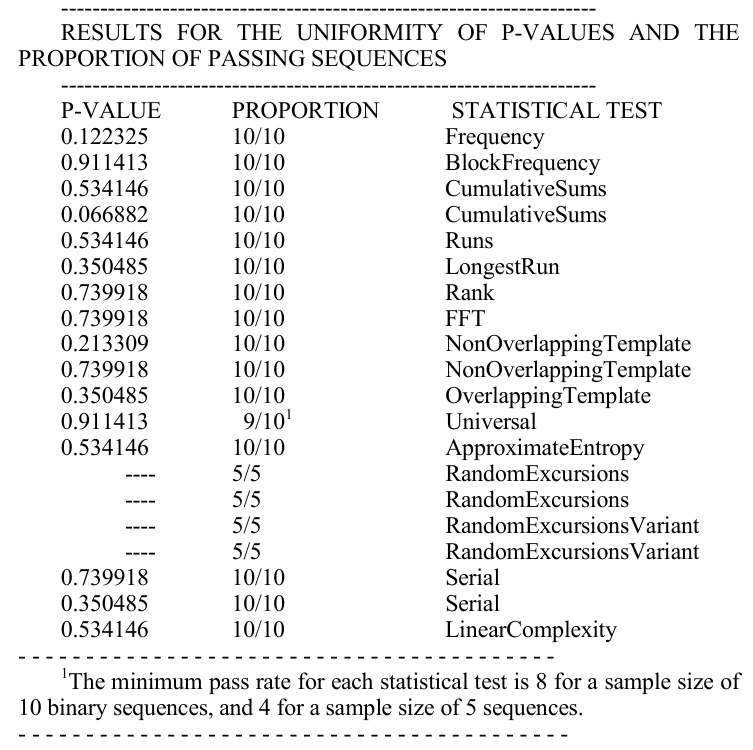
\includegraphics[width=5in]{figs/nist_result.png} 
\caption{NIST test suite results for bits with RTN and thermal noise.}
\label{fig:nist_result} 
\vspace{-0.1in}
\end{center} 
\end{figure} 

We also tested random numbers from one bit with only RTN behavior, using multiple bits from up-time and down-time. In this case, we generated ten 200,000-bit sequences from one bit. The data passed all NIST tests with results that are similar to the above case. For the Universal test, which requires a sequence longer than 387,840 bits, we used five 500,000-bit sequences. 

\subsection{Performance}

The throughput of the proposed RNG varies significantly depending on the switching rate of individual bits, sampling speed and environment conditions. Typically, only a small fraction of bits show pure RTN behavior with minimal thermal noise. TABLE~\ref{tab:pure_rtn} shows the performance of Flash chips from four manufacturers. The average throughput ranges from 848 bits/second to 3.37 Kbits/second. Note that the fastest switching trap that can be identified is limited by the reading speed in our experiments.


\begin{table}
  \begin{center}
    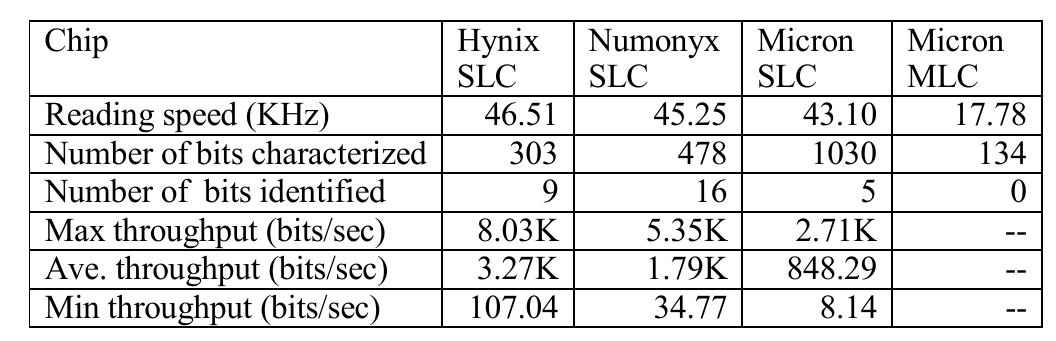
\includegraphics[width=5in]{figs/pure_rtn.png} 
  \end{center}
\caption{Performance of bits with pure RTN behavior.}
\vspace{-0.2in}
\label{tab:pure_rtn}
\end{table}

If bits with both RTN and thermal noise are also used, the percentage of bits which can be used for RNG can be much higher. The performance of these bits from the same Flash chips as in the pure RTN case is shown in TABLE~\ref{tab:rtn_and_thermal}. The average throughputs are higher because thermal noise is high frequency noise.

\begin{table}
  \begin{center}
    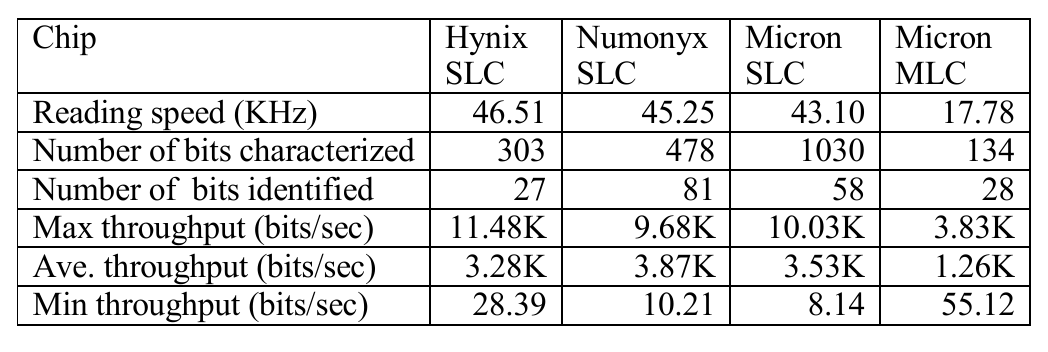
\includegraphics[width=5in]{figs/rtn_and_thermal.png} 
  \end{center}
\caption{Performance of bits with both RTN and thermal noise.}
\vspace{-0.2in}
\label{tab:rtn_and_thermal}
\end{table}

In our tests, the RNG throughput is largely limited by the timing of the asynchronous interface which is controlled by an ARM microcontroller with CPU frequency of 60MHz and the 8-bit bus for a Flash chip. We believe that the RNG performance can be much higher if data can be transferred more quickly through the interface. As an example, the average for RTN transition time is reported to range from 1 microsecond to 10 seconds \cite{abe2011understanding}. If a 128 bytes can be read in 6 microseconds which is the ideal random cache read speed for the Micron SLC chips, a RTN bit with 0.1ms average transition time will give approximately 20 Kbits/second throughput. Note that one page could have multiple RTN bits and our algorithm allows using multiple bits in parallel so that the aggregated throughput of an RNG can be much higher. For example, if N bits can be read at a time, in theory, that can increase the throughput by a factor of N. 

\subsection{Temperature Variations}

For traditional hardware RNGs, low temperatures present a particular challenge because thermal noise, which they typically rely on, can be reduced with the temperature. To study the effectiveness of the Flash-based RNG in low temperatures, we tested the scheme at two low temperature settings: one in a freezer, which is about -5°C, and the other in dry ice, which is about -80°C. The generated random sequences are tested individually as well as combined together with data from experiments at room temperature. All of them passed the NIST test suite without a problem, showing that our technique is effective at low temperatures.

Note that the experiments for temperature variations and aging are performed with a setup where data from Flash memory are transferred from a testbed to a PC through an USB interface. The post processing is performed on the PC. The USB interface limits the Flash read speed to 6.67KHz. As a result, the throughput in this setup is noticeably slower than the results in previous subsections where the entire RNG operation is performed on a microcontroller.  

To understand the impact of temperature variations on the Flash-based RNG, we tested the first 80 bits of a page from a Numonyx chip. At room temperature, 62 bits out of the 80 bits showed oscillations between the programmed state and erased state. 14 bits out of the 62 bits were selected by the selection algorithm, which identifies bits with pure RTN or both RTN and thermal components. The throughputs of the 14 bits are shown in Figure~\ref{fig:throughput_room_temp}. 

Figure~\ref{fig:throughput_m5_temp} and Figure~\ref{fig:throughput_m80_temp} show the performance of the RNG at -5 °C and -80 °C, respectively. At -5 °C, 79 bits out of 80 bits showed noisy behavior and 20 out of 79 bits were selected by the RNG algorithm as ones with RTN. At -80 °C, 72 bits out of 80 bits showed noise and 28 out of 72 bits were selected as the ones with RTN. On average, we found that per-bit throughput is slightly decreased at low temperatures, most likely because of reduced thermal noise and possibly because of slowed RTN switching. However, the difference is not significant. In fact, a previous study \cite{scofield2000temperature} claimed that RTN is temperature independent below 10 Kelvin. Interestingly, we found that the number of bits that are selected by our algorithm as ones with RTN behavior increases at a low temperature. This trend is likely to be because the low temperature decreases thermal noise amplitude while RTN amplitude stays almost the same and the RTN traps slow down so that they become observable at our sampling frequency. 

\begin{figure}
\begin{center} 
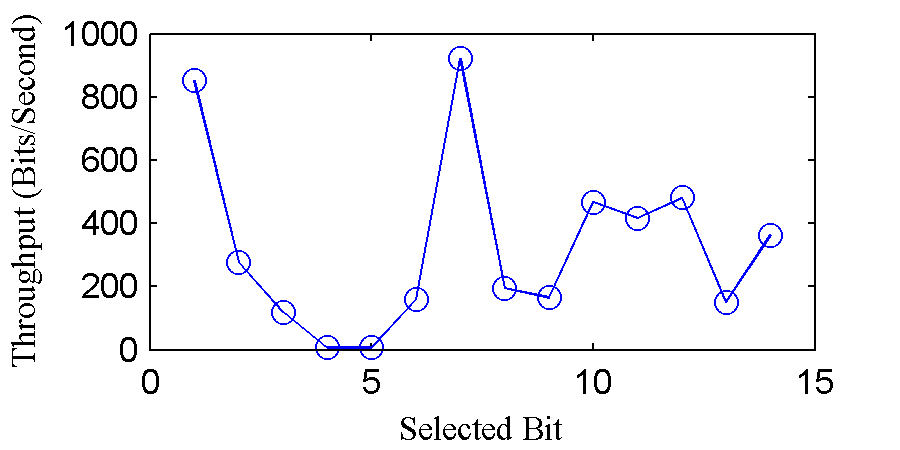
\includegraphics[width=\mywidth]{figs/throughput_room_temp.png} 
\caption{Throughputs under room temperature.}
\label{fig:throughput_room_temp} 
\vspace{-0.1in}
\end{center} 
\end{figure} 

\begin{figure}
\begin{center} 
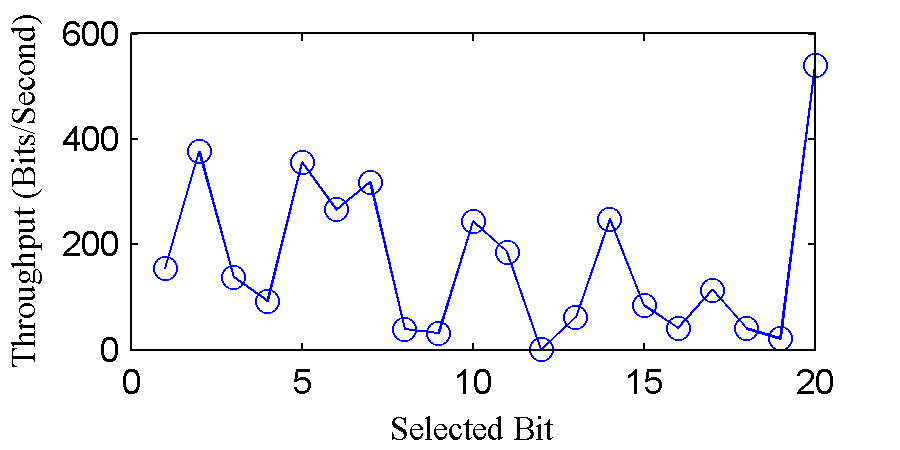
\includegraphics[width=\mywidth]{figs/throughput_m5_temp.png} 
\caption{Throughput at -5 °C.}
\label{fig:throughput_m5_temp} 
\vspace{-0.1in}
\end{center} 
\end{figure} 

\begin{figure}
\begin{center} 
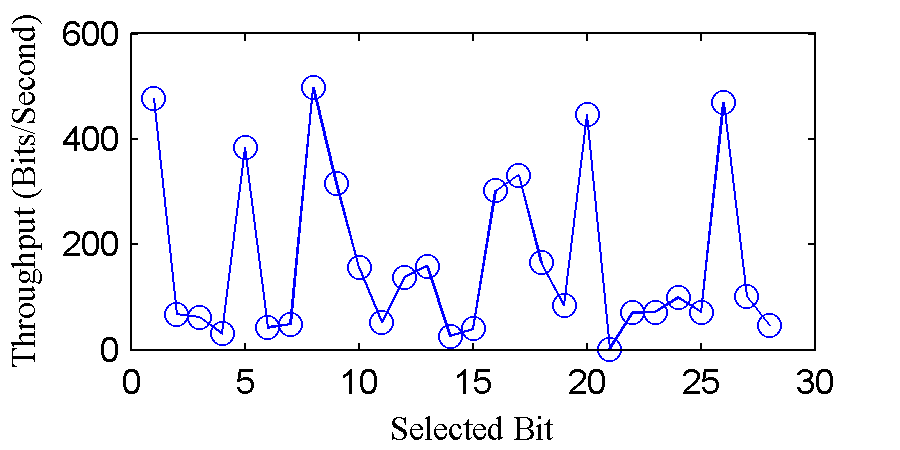
\includegraphics[width=\mywidth]{figs/throughput_m80_temp.png} 
\caption{Throughputs at -80 °C.}
\label{fig:throughput_m80_temp} 
\vspace{-0.1in}
\end{center} 
\end{figure} 

\subsection{Aging}

Flash devices wear-out over time as more program/erase (P/E) operations are performed. A typical SLC Flash chip has a lifetime of 1 million P/E cycles. In the context of RNGs, however, we do not think that wear-outs cause concerns. In fact, aging can create new RTN traps and increase the number of bits with RTN. To check the impact of aging on the RNG, we tested the scheme after 1,000 P/E operations and 10,000 P/E operations as shown in TABLE~\ref{tab:rtn_aging}. The RNG outputs passed the NIST test suite in both cases and did not show any degradation in performance. 

\begin{table}
  \begin{center}
    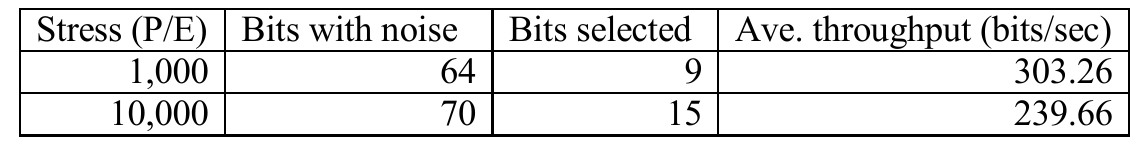
\includegraphics[width=5in]{figs/rtn_aging.png} 
  \end{center}
\caption{Performance summary of RTN in stressed pages}
\vspace{-0.2in}
\label{tab:rtn_aging}
\end{table}

The table shows an interesting trend that more bits show RTN behavior after 10,000 P/E cycles. The increase in noisy bits can potentially increase the overall RNG throughput. One possible concern with aging is a decrease in “stable time period” during which each bit shows noisy behavior. In our experiments, we found that a bit can be used for random number generation for over 12 hours after one programming (Algorithm III). If a bit is completely worn out, charge can leak out more quickly, requiring more frequent calibration. However, given that Flash memory is designed to have a retention time of 10 years within its lifetime, we do not expect the leakage to be a significant problem. We plan to perform larger scale experiments to understand how often a bit needs to be re-programmed for reliable random number generation. In practice, a check can also be added to ensure that a bit oscillates between 1 and 0. 

\section{Application Scenarios}

This section briefly discusses how the Flash memory based security functions, namely RNGs and device fingerprints, can be used to improve security of electronic devices. We first discuss where the techniques can be deployed and present a few use cases. 

The proposed Flash-based security techniques work with commercial off-the-shelf Flash memory chips using standard interfaces. For example, our prototype design is based on the Open NAND Flash Interface (ONFI) \cite{onfi}, which is used by many major Flash vendors including Intel, Hynix, Micron, and SanDisk. Other Flash vendors such as Samsung and Toshiba also use similar interfaces to their chips. 
The proposed techniques can be applied to any Flash or other floating-gate non-volatile memory, as long as one can control read, program (write), and erase operations to specific memory locations (pages and blocks), issue the RESET command and disable internal ECC. Embedded systems typically implement a Flash memory controller in software, exposing the low-level Flash chip interface to a software layer. Our prototype USB board in the evaluation section is an example of such a design. While we did not have a chance to study details, the manual for the TI OMAP processor family \cite{instruments2013omap}, which is widely used in mobile phones, indicates that its External Memory Interface (EMI) requires software to control each phase of NAND Flash accesses. In such platforms where Flash accesses are controlled by software, our techniques can be implemented as relatively simple software changes. 

For large memory components such as SSDs, the low-level interfaces to Flash memory chips may not be exposed to a system software layer. For example, SSD controllers often implement wear-leveling schemes that move data to a new location on writes. In such devices, the device vendor needs to either expose the Flash interfaces to higher level software or implement the security functions in firmware.  


The Flash-based random number generator (RNG) can either replace or complement software pseudo random number generators in any applications that need sources of randomness. For example, random numbers may be used as nonces in communication protocols to prevent replays or used to generate new cryptographic keys. Effectively, the Flash memory provides the benefits of hardware RNGs for systems without requiring custom RNG circuits. For example, with the proposed technique, low-cost embedded systems such as sensor network nodes can easily generate random numbers from Flash/EEPROM. Similarly, virtual machines on servers can obtain true random numbers even without hardware RNGs.

\section{Related Work}

Hardware random number generators generate random numbers from high-entropy sources in the physical world. Theoretically, some random physical processes are completely unpredictable. Therefore, hardware random number generators provide better random numbers in terms of randomness than software based pseudo-random number generators.

Thermal noise and other system level noise are the common entropy sources in recently proposed hardware random number generators. In \cite{sunar2007provably}, the phase noise of identical ring oscillators is used as the entropy source. In \cite{o2004puf}, the differences in path delays are used. In \cite{majzoobi2011fpga} and \cite{intelrng}, the metastability of flip-flops or two cross coupled inverters are used. Basically, the entropy source of these RNG designs is thermal noise and circuit operational conditions. These hardware random number generators can usually achieve high throughput because the frequency of the entropy sources is high. One common characteristic of these hardware random generators is that they all need carefully designed circuits where process variations should be minimized so that noises from the entropy source can be dominant. Compared to this, the random number generation in Flash memory cells does not require specially designed circuits and is more immune to process variation. Moreover, our entropy source is based on quantum behavior and theoretically, it should still work under extremely low temperatures where thermal noise or other kinds of noise decrease dramatically.
